\documentclass[10pt,a4paper]{article}
\usepackage[utf8]{inputenc}
\usepackage[english]{babel}
\usepackage{amsmath}
\usepackage{amsfonts}
\usepackage{amssymb}
\usepackage{graphicx}

\usepackage{booktabs}

\begin{document}

\begin{figure}
\centering
\begin{tabular}{c}
\begin{tabular}{cccc}
\multicolumn{4}{c}{\textbf{Grupo CTRL}} \\
MJH & JAE & MGG & EMT \\
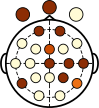
\includegraphics[width=0.17\textwidth]{./img_art_dfa/prop_MJH_30.pdf} &
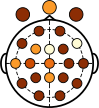
\includegraphics[width=0.17\textwidth]{./img_art_dfa/prop_JAE_30.pdf} &
\includegraphics[width=0.17\textwidth]{./img_art_dfa/prop_MGG_30.pdf} &
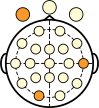
\includegraphics[width=0.17\textwidth]{./img_art_dfa/prop_EMT_30.pdf} \\
\end{tabular} \\
\midrule
\begin{tabular}{ccccc}
\multicolumn{4}{c}{\textbf{Grupo PDCL}} \\
CLO & RLO & JGZ & AEFP & PCM \\
\includegraphics[width=0.17\textwidth]{./img_art_dfa/prop_CLO_30.pdf} &
\includegraphics[width=0.17\textwidth]{./img_art_dfa/prop_RLO_30.pdf} &
\includegraphics[width=0.17\textwidth]{./img_art_dfa/prop_JGZ_30.pdf} &
\includegraphics[width=0.17\textwidth]{./img_art_dfa/prop_AEFP_30.pdf} &
\includegraphics[width=0.17\textwidth]{./img_art_dfa/prop_PCM_30.pdf} \\
\end{tabular}
 \\
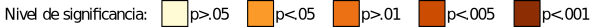
\includegraphics[scale=.7]{./img_art_dfa/escala.pdf} \\
\end{tabular}
\caption{Derivaciones para las cuales la proporción de épocas clasificadas como estacionarias fue significativamente diferente en MOR y NMOR.
%
En la parte superior se representa al grupo CTRL y en la parte inferior al grupo PDCL.
%
Para esta figura se usaron épocas de 30 segundos de duración.
%
La posición de los círculos representan a las derivaciones, en correspondencia con la figura \ref{img:estampa}.}
\label{cabeza_new}
\end{figure}

\end{document}